\subsection{\textsc{SubBytes} transformation}
\label{sec:SubBytes}

The \textsc{SubBytes} transformation is a non-linear byte substitution step that operates independently on each byte of the AES state. 
It can be viewed as the application of 16 parallel S-Boxes, each processing 8-bit input to produce an 8-bit output, as illustrated in Figure~\ref{fig:byte-substitution}. 
For every byte $A_i$ in the \gls{AES} state, the transformation produces a substituted byte $B_i$, defined by the function $B_i = S(A_i)$.

\begin{figure}[!ht] 
    \centering
    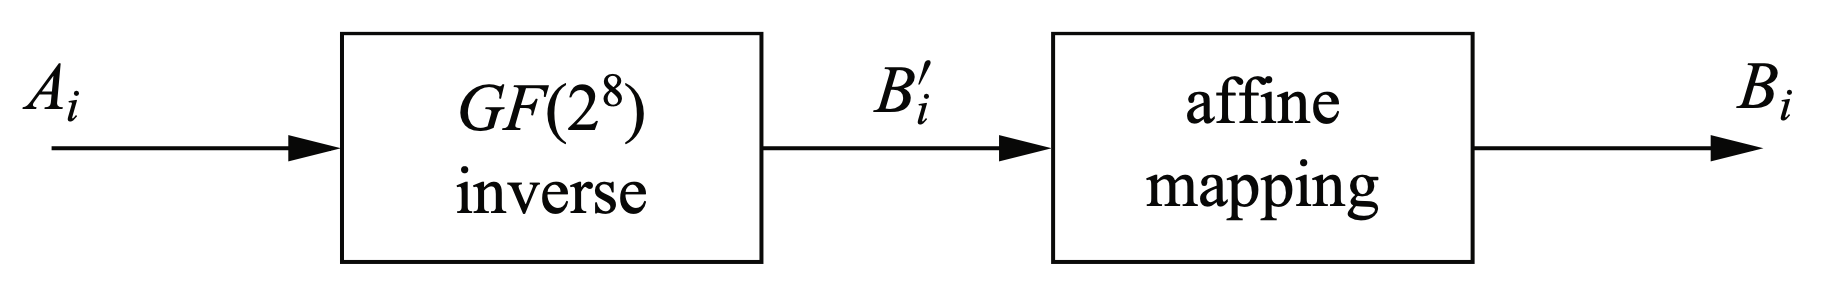
\includegraphics[width=.6\textwidth]{byte-substitution.png} 
    \caption{
        The two operations within the AES S-Box which computes the function $B_i = S(A_i)$ \cite{Paar2024}.
    }
    \label{fig:byte-substitution} 
\end{figure}

The construction of the S-Box is based on two sequential transformations:
\begin{enumerate}
    \item \textbf{Galois Field Inversion}: 
    Each byte is interpreted as an element in the finite field $GF(2^8)$ and is mapped to its multiplicative inverse in this field. 
    This operation is defined by:
    
    \begin{align}
        A_i \cdot {B'}_i &= 1 \mod m(x)
        \label{eq:gfi}
    \end{align}
    where $m(x)$ is the irreducible polynomial defining the field, as discussed in Section~\ref{sec:multiplication}. 

    The element ${00}$, which has no inverse, is mapped to itself.

    \item \textbf{Affine Mapping}:
    
    Each resulting byte ${B'}_i$ undergoes a bitwise affine transformation over $GF(2)$. 
    This transformation is defined as:
    \begin{align}
        b_i = {b'}_i \oplus {b'}_{(i+4 \mod 8)} \oplus {b'}_{(i+5 \mod 8)} \oplus {b'}_{(i+6 \mod 8)} \oplus {b'}_{(i+7 \mod 8)} \oplus c_i
    \end{align}
    for $0 \leq i \leq 8$, where $b_i$ is the $i$-th output bit of the byte, ${b'}_i$ are the bits of the inverted byte, and $c_i$ are bits from a fixed constant byte.
\end{enumerate}

A complete S-Box can be precomputed by applying these transformations to all 256 possible input bytes (from \texttt{00} to \texttt{FF}), allowing efficient lookup during AES encryption. 
The full substitution table is shown in Figure~\ref{fig:sbox}.

\begin{figure}[!ht]
    \centering
    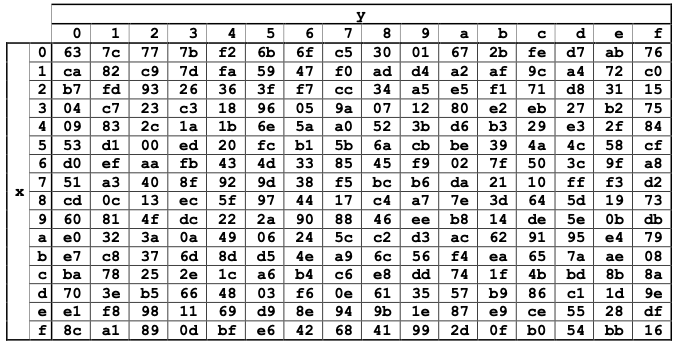
\includegraphics[width=.8\textwidth]{sbox.png}
    \caption{S-Box: substitution values for the byte $\{xy\}$ \cite{NIST_AES}.}
    \label{fig:sbox}
\end{figure}


\paragraph{Example:} \textsc{SubByte} transformation of $(53)_{\text{hex}}$

\begin{equation}
    \textsc{SubByte}((53)_{\text{hex}}) = (ed)_{\text{hex}}
\end{equation}
